%----------------------------------------------------------------
%
%  File    :  chapter5.tex
%
%  Authors :  Michael Fuska, FH Campus Wien, Austria
% 
%  Created :  08 Feb 2016
% 
%  Changed :  
% 
%----------------------------------------------------------------
\chapter{iOS Sicherheitskonzepte}
\label{ch:iOSSicherheitsKonzepte}

%------------------------------------------------------------------------------
%------------------------------ Reduziertes Betriebsystem
\section{Reduziertes Betriebsystem}
\label{sec:reduziertesOS}
Unter iOS wurden die Angriffsvektoren für Hacker reduziert, indem das mobile Betriebssystem reduziert wurde. Der User hat nicht die Möglichkeit, auf den internen Flash Speicher des Gerätes zuzugreifen. Weder über einen File-Explorer noch über ein Terminalprogramm. 
\begin{description}
    \item[\parbox{\textwidth} {Unter anderem sind folgende Terminalprogramme unter iOS nicht verfügbar}]~\par
    \begin{itemize}
       \item telnet
       \item ssh
    \end{itemize}
\end{description} 
Auf einen Device mit Jailbreak, können beide Terminalprogramme und verschiedenste File-Explorer installiert werden. Somit kann der User die Daten des iOS Device verwalten.(lesen, schreiben, löschen und ändern)
\begin{description}
    \item[\parbox{\textwidth} {Aus Sicherheitsgründen sind folgende Dienste/Entwicklungsumgebungen nicht installiert}]~\par
    \begin{itemize}
       \item Java
       \item Shell Programme (bash, sh, csh, usw.)
       \item Adobe Flash
    \end{itemize}
\end{description} 

%------------------------------------------------------------------------------
%------------------------------  Memory Protection
\section{Memory Protection Mechanism}
\label{sec:MemoryProtection}
Die wichtigsten \textbf{Memory Protection Mechanismen} unter iOS sind
\begin{enumerate}
    \item \textbf{Secure Boot Chain}
    \item \textbf{Address Space Layout Randomization (ASLR)}
    \item \textbf{Mandatory Access Control (MAC)}
\end{enumerate}

% -------------------------
%------------------------------ Secure boot chain
\subsection{Secure Boot Chain}
\label{sec:SecBootChain}

Die \textbf{Secure Boot Chain} ist eine Kernsicherheit Funktionalität des iOSs. Jede Phase des Boot-Prozesses ist verschlüsselt. Jedes Module/Phase enthält den Key zum Entschlüsseln der nächsten Phase. Dadurch ist sichergestellt, dass die Boot Kette nicht unterbrochen wird. \par

Der \textit{\glqq Boot Read Only Memory (ROM)\grqq{}} ist der \textit{\glqq Root of Trust\grqq{}} vom der Secure Boot Chain. Im ersten Step wird das \textit{\glqq Root Zertifikat\grqq{}} aus dem ROM gelesen. Das Root Zertifikat wurde durch die \textit{\glqq Apple Certificate Authority (CA)\grqq{}} signiert. Der öffentliche Schlüssel des Root Zertifikates wird verwendet, um die Signatur des Low Level Boot Loaders zu prüfen. Wenn die Signatur erfolgreich validiert wurde, wird der LLB mit dem Key aus dem ROM entschlüsselt und geladen. Diese Schritte werden für jedes Modul/Phase des Secure Boot Chain durchgeführt. Diese Vorgangsweise  wird Secure Boot Chain genannt.

\begin{description}
    \item[\parbox{\textwidth}{Die Secure Boot Chain beinhaltet folgende Module/Phasen}]~\par
   \begin{enumerate}
        \item \textbf{Low Level Bootloader (LLB)},
        \item \textbf{iBoot},
        \item \textbf{Kernel},
        \item \textbf{Kernel Extension}
        \item \textbf{Baseband Firmware}.
    \end{enumerate}
\end{description} 

Die Secure Boot Chain stellt sicher, dass keine Veränderung der Hardware und/oder des iOS Kernels, während des Boot Prozesses vorgenommen werden kann. Nach erfolgreicher Verifikation der Kernel Signatur, wird der Kernel entschlüsselt und das mobile Betriebsystem von Apple wird geladen. In nächsten Schritt wird die Signatur jedes Prozesses, sowohl vom Betriebssystem, als auch von den User Applikationen validiert. Nur wenn die Prüfung der Signatur erfolgreich war, wird der Code und die Libraries in den Memory des iOS Devices geladen. Dies stellt sicher, dass nur eine Software auch einem iOS Gerät geladen werden kann, welche mit einem gültigen Zertifikat signiert wurde. (vgl. \cite{Apple[4], Apple[5], Apple[6]})

% -------------------------
% -------------------------
%\subsection{Boot ROM}
%\label{sec:BootROM}
%% http://resources.infosecinstitute.com/understanding-ios-security-part-1/
%
%% -------------------------
%% -------------------------
%\subsection{Low Level Boot Loader}
%\label{sec:LowLevelBootLoader}
%
%% -------------------------
%% -------------------------
%\subsection{iBoot}
%\label{sec:iBoot}
%
%% -------------------------
%% -------------------------
%\subsection{Kernel}
%\label{sec:Kernel}
%
%------------------------------------------------------------------------------
%------------------------------ Secure Recovery Boot Chain
%\section{Secure Recovery Boot Chain}
%\label{sec:SecureRecoveryBootChain}

%\subsection{Recovery Mode}
%\label{sec:RecoveryMode}

% -------------------------
% -------------------------
\subsection{Address Space Layout Randomization (ASLR)}
\label{sec:ASLR}

Durch die Implementierung von \textbf{Address Space Layout Randomization (ASLR)} wurde die Exploitation von Softwarebugs unter iOS erheblich schwerer. ASLR hat die Aufgabe beim Starten des Betriebssystems und der Programme diesen randomisierte Memory Adressen zuzuweisen. Dadurch ist die Zuweisung der Speicheradressen nicht mehr deterministisch. Wenn ASLR im vollen Funktionsumfang implementiert worden ist, muss ein Hacker mehrere Softwarefehler finden um einen Memory Exploitation ausnützen zu können. Betriebssysteme die ASLR nur teilweise implementiert haben, ermöglichen es Hackern Memory Bereiche zu lokalisieren bzw vorherzusagen die \textit{\glqq writable\grqq{}} oder \textit{\glqq executable\grqq{}} sind und somit können diese Systeme leichter angegriffen werden. (vgl. \cite{Apple[4], ASLR[1], ASLR[2]}) \par

Das mobile Betriebssystem von Apple unterstützt ASLR seit der iOS Version 4.3. Jede App hat die Möglichkeit diesen Mechanismus mit dem Compiler Flag \textbf{Position Independent Executables (PIE)} zu aktivieren. Wenn die App mit dem PIE Flag kompiliert wurde, dann werdem
\begin{itemize}
    \item \textbf{dem Base Pointer(EBP),}
    \item \textbf{dem Textsegment,} 
    \item \textbf{dem Datensegment,}
    \item \textbf{dem BSS Segment,} 
    \item \textbf{dem Stack Segment,}
    \item \textbf{dem Heapsegment}
    \item \textbf{und den Libraries der App}
\end{itemize}
unterschiedliche \textit{\glqq virtual Memory-Adressen\grqq{}} zugewiesen. Alle unter iOS vorinstallierten Apps wurden mit diesem PIE Flag kompiliert. 

Die nachfolgenden Tabellen \ref{tab:PIE executable segment}, \ref{tab:PIE data segment}, \ref{tab:PIE stack segment}, \ref{tab:PIE heap segment}, \ref{tab:PIE libraries} und \ref{tab:PIE linker } zeigen die PIE Variationen

 \begin{table}
    \begin{center}
         \begin{tabular}{|p{6cm}|p{9cm}|} \hline
            Compiling Option PIE ist gesetzt & Code Segment \\ \hline
            Nein & fixe Memory Adresse\\ \hline
            Ja & randomisierte Memory Adresse per Ausführung (execution)\\ \hline
        \end{tabular}
        \caption{PIE executable segment (vgl. \cite{iOSSec[5]}) }
       \label{tab:PIE executable segment}
    \end{center}
\end{table}

 \begin{table}
    \begin{center}
       \begin{tabular}{|p{6cm}|p{9cm}|} \hline
            Compiling Option PIE ist gesetzt & data segment\\ \hline
            Nein & fixe Memory Adresse\\ \hline
            Ja & randomisierte Memory Adresse per Ausführung (execution)\\ \hline
        \end{tabular}
        \caption{PIE data segment (vgl. \cite{iOSSec[5]})}
       \label{tab:PIE data segment}
    \end{center}
\end{table}

\begin{table}
    \begin{center}
        \begin{tabular}{|p{6cm}|p{9cm}|} \hline
            Compiling Option PIE ist gesetzt & Stack Segment\\ \hline
            Nein & fixe Memory Adresse\\ \hline
             Ja & randomisierte Memory Adresse per Ausführung (execution)\\ \hline
        \end{tabular}
         \caption{PIE stack segment (vgl. \cite{iOSSec[5]})}
       \label{tab:PIE stack segment}
    \end{center}
\end{table}    

\begin{table}
    \begin{center}
       \begin{tabular}{|p{6cm}|p{9cm}|} \hline
            Compiling Option PIE ist gesetzt & Heap Segment\\ \hline
            Nein & randomisierte Memory Adresse per Ausführung (execution)\\ \hline
            Ja & randomisierte Memory Adresse per Ausführung (execution)\\ \hline
        \end{tabular}
        \caption{PIE heap segment (vgl. \cite{iOSSec[5]}) }
       \label{tab:PIE heap segment}
    \end{center}
\end{table}

\begin{table}
    \begin{center}
      \begin{tabular}{|p{6cm}|p{9cm}|} \hline
            Compiling Option PIE ist gesetzt & Libraries \\ \hline
            Nein & Randomisierte Memory Adresse per Device boot\\ \hline
            Ja & Randomisierte Memory Adresse per Device boot \\ \hline
        \end{tabular}
        \caption{PIE libraries (vgl. \cite{iOSSec[5]})}
       \label{tab:PIE libraries}
    \end{center}
\end{table}

 \begin{table}
    \begin{center}
        \begin{tabular}{|p{6cm}|p{9cm}|} \hline
            Compiling Option PIE ist gesetzt & Linker  \\ \hline
            Nein & fixe Memory Adresse\\ \hline
            Ja & Randomisierte Memory Adresse per Ausführung (execution)\\ \hline
        \end{tabular}
        \caption{PIE linker (vgl. \cite{iOSSec[5]})}
       \label{tab:PIE linker }
    \end{center}
\end{table}

% -------------------------
% -------------------------
\subsection{Mandatory Access Control}
\label{sec:MAC}

 \textbf{Mandatory Access Control (MAC)} ist ein Konzept zur Kontrolle und Steuerung von Zugriffsrechten. MAC überprüft jeden ausführbaren Code und jede Library, die in den Memory geladen werden sollten. Im Gegensatz dazu prüft \textbf{Data Execution Prevention (DEP)} nur Binaries. iOS erfährt somit einen deutlichen Sicherheitsgewinn gegenüber anderen mobilen Betriebssystemen. \par 
 MAC wurde mit der iOS Version 2.0 eingeführt. Bis zum heutigen Zeitpunkt gibt es keinen Weg um diese Zugriffskontrolle zu umgehen. Von jedem ausführbaren Code und jeder Library wird die Signatur geprüft, bevor die Daten in den virtuellen Memory geladen werden. (vgl. \cite{iOSSec[5], Hacking[1]})
Der MAC Mechanismus hat zwei Vorteile gegenüber anderen Memory Protection Systemen. \par 
Erstens Malware kann auf einem iOS Gerät nur ausgeführt werden, wenn diese auch zuvor von einem gültigen Zertifikat signiert worden ist. Es gibt Bespiele in denen es Hackern gelungen ist, die Malware in einer App so zu verstecken, dass die App offiziell von Apple signiert worden ist. Dies konnte erreicht werden, in dem Malware in Code Branches versteckt wurde, die in dem normalen Codefluss der App nie durchlaufen wird. (vgl. \cite{iOSSec[5], Hacking[1]}) \par
 Der zweite Vorteil ist, dass die Exploits nur unter Anwendung von \textit{ \glqq Return Oriented Programming(ROP)\grqq{} } durchgeführt werden können. ROP ist weit aus komplexer, als normale Shell Code Exploits.(vgl. \cite{Architecture[1], Architecture[2], Architecture[3], ROP[1], ROP[2], iOSSec[5], Hacking[1]})

MAC wurde unter iOS im \textbf{Mandatory Access Control Framework(MACF)} implementiert. Für iOS wurden zwei \textit{\glqq mandatory access control policies\grqq{}} konfiguriert
\begin{enumerate}
   \item Sandbox (Siehe Kapitel \ref{sec:Sandbox})
   \item AMFI (Siehe Kapitel \ref{sec:AMFI})
\end{enumerate}
(vgl. \cite{iOSSec[5], Hacking[1]})

% -------------------------
% -------------------------
\subsubsection{Apple Mobile File Integrity (AMFI)}
\label{sec:AMFI}
\textbf{AMFI } ist eine Kernel Extension die den Code Signing Sicherheitsmechanismus implementiert hat. Die \textbf{AMFI Kernel Extension} überprüft die Signatur von jedem ausführbaren Code und von jeder Library. Sollten die Signatur (CDHash) nicht durch die AMFI Kernel Extension validiert werden können, wird über ein \textit{\glqq Remote Procedure Call (RPC) Interface\grqq{}} (Userspace) versucht, der Prozess zu validieren. Folgende Programmschnittstellen (Hooks) stehen der AMFI Kernel Extension für die Validierung der Signatur zur Verfügung

\begin{itemize}
    \item \label{item:AMFIfunc} \textbf{mpo\_vnode\_check\_signature:} \\
    Dieser Funktion wird als Parameter der CDHash übergeben und es wird überprüft ob der CDHash im \textbf{static} oder \textbf{dynamic trust cache} eingetragen ist. Wenn nicht, muss der CDHash über das RPC Interface validiert werden. (Siehe Kapitel: \ref{sec:SignediOSApp}) (vgl. \cite{iOSSec[5], Hacking[1]})
    \item \textbf{mpo\_vnode\_check\_exec:}\\
    Diese Funktion setzt die Flags CS\_HARD und CS\_KILL in der \textit{\glqq proc-Struktur\grqq{}} des Prozess. (vgl.\cite{iOSSec[5],  Hacking[1]})
    \item \textbf{mpo\_proc\_check\_get\_task:}\\
    Diese Funktion prüft die Entitlements get-task-allow and task\_for\_pid-allow. Wenn beide gesetzt sind hat der Prozess Zugriff auf den \textit{\glqq Task Control Port\grqq{}}. Damit erhält  die App Zugriff auf die Debug-Informationen des Systems. (vgl. \cite{iOSSec[5],  Hacking[1]})
    
    \item \textbf{mpo\_proc\_check\_run\_cs\_invalid:} \\
    Mit diesem Hook kann definiert werden, ob ein Programm ausgeführt werden darf, auch wenn das System festgestellt hat, dass dieses Programm nicht vertrauenswürdig ist. Dieser Fall kann eintreten, wenn das Programm nicht überprüft werden konnte oder der Code verändert wurde. Hierfür müssen die Entitlements 
    \begin{itemize}
        \item get-task-allow, 
        \item run-invalid-allow 
        \item und run-unsigned-code 
     \end{itemize} 
     gesetzt sein. (vgl. \cite{iOSSec[5]} S.5, \cite{Hacking[1]})
    
    \item \textbf{mpo\_proc\_check\_map\_anon:}\\
    Nur in dem Fall, wenn der Prozess das Dynamic Code Signing Entitlement gesetzt hat kann der Prozess anonymous Memory allokieren. (vgl. \cite{iOSSec[5],  Hacking[1]})
\end{itemize}

Die AMFI Kernel Extension setzt die \textit{\glqq csflags\grqq{}} in der \textit{\glqq proc-Struktur\grqq{}} jedes Prozesses. Bei der Allokation und der Verwaltung der virtuelle Memory Pages werden die csflags des Prozess  vom Kernel überprüft. Diese Funktionalität ist das Bindeglied zwischen der Signatur/Entitlements der App und der virtuellen Speicherverwaltung des iOS Devices. 

%Thus, the kernel knows whether the process is successfully validated or not. The Table \ref{tab:CSFLAGS} describes the possible values of the csflags that can be set by the amfi kernel extension. \cite{iOSSec[5], Hacking[1]}
Alle definierten \textit{\glqq csflags\grqq{}} werden in der Tabelle: \ref{tab:CSFLAGS} angeführt.
\begin{table}[ht]
\begin{center}
\begin{tabular}{|l|c|p{8cm}|} \hline
  Flag Name & Value & Beschreibung\\ \hline
CS\_VALID & 0x00001 & Der Prozess ist dynamisch \textit{\glqq valid\grqq{}} \\ \hline
CS\_HARD & 0x00100 & Der Prozess darf keine \textit{\glqq invalid Page\grqq{}} laden.\\ \hline
CS\_KILL & 0x00200 & Der Prozess sollte \textit{\glqq beendet\grqq{}} werden, wenn der Prozess dynamisch \textit{\glqq invalid\grqq{}} werden würde.\\ \hline
CS\_EXEC\_ SET\_HARD & 0x01000 & Der Prozess setzt das CS\_HARD Flag für jeden ausgeführten Childprozess.\\ \hline
CS\_EXEC\_ SET\_KILL & 0x02000 & Der Prozess setzt das CS\_KILL Flag für jeden ausgeführten Childprozess. \\ \hline
CS\_KILLED & 0x10000 & Der Process wurde vom Kernel \textit{\glqq beendet\grqq{}} bevor dieser dynamisch \textit{\glqq invalid\grqq{}} ist.\\ \hline
\end{tabular} 
\caption{Value \textit{\glqq csflags\grqq{}} (vgl. \cite{iOSSec[5]} S.11)}
\label{tab:CSFLAGS}
\end{center}
\end{table}


\paragraph{Zusammenfassend:} Es gibt drei Möglichkeiten für die AMFI Kernel Extension die Signatur(CDHash) einer App zu validieren
\begin{enumerate}
    \item \textbf{Static trusted cache:} \\
    In diesem permanenten Speicher werden alle CDHash gespeichert, die fixer Bestandteil des mobilen Betriebssystems von Apple sind.  
    \item \textbf{Dynamic trusted cache:} \\
    Dies ist ein dynamischer Speicher in dem alle CDHashes gespeichert werden, die schon einmal erfolgreich verifiziert wurden. Mit jedem Neustart des Devices wird dieser Speicher neu initialisiert.
    \item \textbf{AMFI RPC Interface} 
\end{enumerate}   
  
 Aus sicherheitstechnischen Gründen wurde die Verifizierung des CDHash vom \textit{\glqq Kernelspace\grqq{}} in den \textit{\glqq Userspace\grqq{}} ausgelagert. Damit werden die sehr komplexen und teuren kryptographische Rechenoperationen nicht mehr im sicherheitskritischen Kernelspace durchgeführt. Die Kommunikation zwischen der AMFI Kernel Extension (Kernelspace) und dem \textit{\glqq amfid Dämon (Userspace)\grqq{}} findet über die Remote Prozedur Calls(RPC) statt. Für diese Interprozesskommunikation stehen zwei Prozeduren zur Verfügung. Diese werden im Table \ref{tab:AMFID} beschrieben. (vgl. \cite{iOSSec[5]} S.13, \cite{Mach[1]}) 

\begin{table}[ht]
\begin{center}
\begin{tabular}{|c|p{8,5cm}|} \hline
  Funktion & Beschreibung\\ \hline
verify\_code\_directory &  
Diese Funktion überprüft den CDHash und die Signatur der App. Es wird die Gültigkeit und die Vertraulichkeit der Signatur überprüft. Die Grundlage für diese Prüfung das Apple Zertifikate(ROM) und das mit der App installierte Provisioning Profiles.\\ \hline

permit\_unrestricted\_ debugging &  
Diese Funktion überprüft die UDIDs der Provisioning Profiles des iOSs. Die Provisioning Profiles wurden mit den Apps auf dem iOS Device installiert. Es wird geprüft, ob für die UDID ein uneingeschränktes Debugging erlaubt ist. \\ \hline
\end{tabular} 
\caption{AMFI Daemon Mach RPC Interface (vgl. \cite{iOSSec[5]} S.13)}
\label{tab:AMFID}
\end{center}
\end{table}

% -------------------------
% -------------------------
\subsubsection{Virtual Memory Pages}
\label{sec:virMemoryPages}
 Als \textbf{virtual Memory} wird die Technik bezeichnet, die den \textit{\glqq Adressraum\grqq{}} eines Prozesses unabhängig vom physischen Arbeitsspeicher des iOS Devices macht. Der Begriff \textbf{Paging} bezeichnet die Abbildung der virtuellen Adressen auf die physischen.\par 
Unter iOS gibt es zwei verschiedene Typen von virtuellen Memory Pages, die sich in den gesetzten Permissions unterscheiden 

\begin{enumerate}
    \item Lese- (read) und Schreibzugriff (write)
    \item Lesezugriff (read) und ausführbarer Zugriff (execute)
\end{enumerate}
Diese Permissions verhindern, dass der Inhalt des Speichers nach dem Laden verändert werden kann. Ein weiterer Vorteil ist, dass das Erzeugen von \textit{\glqq neuen dynamischem Code\grqq{}} unterbunden wird. iOS macht  nur für einige Apps/Prozesse eine Ausnahme von dieser Regel. Der \textit{\glqq MobileSafari Webbrowser\grqq}, ist einer dieser Apps und kann zur Laufzeit \textit{\glqq dynamische HTML Seiten\grqq{}} generieren (Java Script). (Just in Time(JIT) Kapitel: \ref{sec:Jit}).


%CSE is built into the iOS kernel’s virtual memory system and most of its implementation is visible in Apple’s open source xnu kernel7, which is shared between iOS and Mac OS X. In essence, the virtual memory system tracks the validity of executable memory Pages and the process as a whole using the “dirty” bit used to implement Copy-on-Write (COW) semantics and virtual memory Pages -ins. When an executable memory Pages is Pages d-in and is marked as being “dirty”, its signature may have been invalidated and it must be reverified. New executable memory Pages are always “dirty”. If a single memory Pages is found to be invalid, then the entire process’ code signing validity is also set to be invalid.
%The code signing validity of the process is tracked with the CS_VALID flag in the csflags member of the kernel’s proc structure for that process. If the executable’s code signing signature has been validated prior to it being executed, the process begins execution with the CS_VALID flag set. If the process becomes invalid, then this flag will be cleared. What happens next depends on the CS_KILL flag. If this flag is set, the kernel will forcibly kill the process once it becomes invalid. On Mac OS X, the default is to not set this flag so that processes created from signed binaries may become invalid. On iOS, however, this flag is set by default so the process is killed once it becomes invalid. The flags defined for this field and a system call (csops) for getting and setting them from user space are documented in bsd/sys/codesign.h. The defined flags are also summarized in the table below:

% -------------------------
% -------------------------
\subsubsection{Dynamisches Code Signing (DCS)}
\label{sec:Jit}

Mit der iOS Version 2.0 wurde \textbf{Dynamisches Code Signing (DCS)} eingeführt, um den Performanz-Ansprüchen der User gerecht zu werden. Es wurden in den unterschiedlichen iOS Versionen immer wieder DCS-Bugs behoben, bis die endgültige DCS-Version in iOS Version 4.3 veröffentlicht wurde. 
\paragraph{Just In Time (JIT)} wird unter iOS mit Hilfe von DCS ermöglicht. Der JIT-Kompiler übersetzt zur Laufzeit das Programm in Bytecode. Der Bytecode wird in einen bestimmten Speicher geschrieben und ausgeführt. Somit muss es auch unter iOS einen Speicherbereich im virtual Memory geben, der sowohl beschreibbar als auch ausführbar ist.  JIT ist aber aus Sicherheits- und Performanz-Gründen auf einige wenige Anwendungen beschränkt. Weiter wird sichergestellt, dass immer nur ein Prozess Zugang zu einem schreib- und ausführbaren Memory Bereich hat. Nur Prozesse die das Entitlement \textbf{dynamic-codesigning} (Siehe Abbildung: \ref{fig:JIT}) gesetzt haben, können JIT verwenden und diesen speziellen Speicherbereich anfordern. Dadurch kann JavaScript im MobileSafari Webbrowser verwendet werden. (vgl. \cite{JIT[1]})

Es werden für eine JIT Request immer 16MB an Speicher reserviert. Der Kernel setzt nach der Prüfung der Entitlement, der Signatur und der Prüfung, ob dieser Prozess JIT verwenden darf, die entsprechenden Berechtigungen(RWX) im Virtual Memory.

\begin{figure}[htp!]
        \centering
                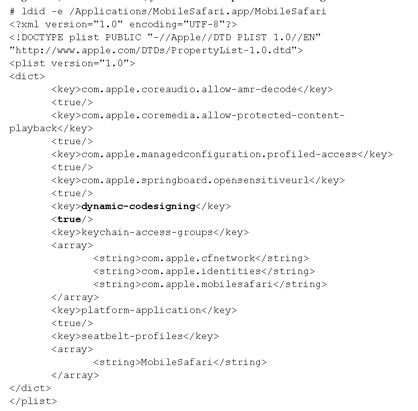
\includegraphics[scale=0.8]{JIT}
        \caption{Just in Time Entitlement (vgl. \cite{Hacking[1]}) }
        \label{fig:JIT}
\end{figure}
% -------------------------
% -------------------------
\section{Signieren von Apps}
\label{sec:SigningProcess}

Apple führte mit der iOS Version 2.0 \textit{\glqq das verpflichtende Signieren von Apps\grqq{}} ein, um ausführbaren Code und Libraries zur Laufzeit zu prüfen. Das Signieren einer App verhindert, dass 
\begin{itemize}
    \item \textbf{unsignierte Libraries,
}    \item \textbf{neuer Code zur Laufzeit,} 
    \item \textbf{und/oder selbstmodifizierender Code geladen und ausgeführt wird.}
\end{itemize}
Jede App wird mit einem Zertifikat signiert. Dadurch wird eine digitale Identität einer App zuzuordnen. (vgl. \cite{Cert[2], Cert[3]}).
\begin{description}
    \item[\parbox{\textwidth} {Eine App kann auf zwei Arten signiert werden}]~\par
   \begin{enumerate}
        \item Die Apps werden mit den Apple Root-Zertifikat signiert und mit Hilfe von iTunes verteilt. 
        
        \item Apple autorisiert \textit{\glqq Third Parties\grqq}, dadurch können Unternehmen ihre Apps selbst signieren und verteilen. Die Verteilung der App kann dadurch in einem geschlossenen Userkreis stattfinden. Mit der App wird auch das entsprechende \textit{\glqq Provisioning Profile\grqq{}} (Siehe Kapitel: \ref{sec:ProvisioningProfile}) verteilt.
    \end{enumerate} 
\end{description} 
(vgl. \cite{Sign[1], Sign[2], Sign[3], Sign[4], Sign[5], ROP[1]}) \par 
Die Signatur der App wird von der AMFI Kernel Extension (Siehe Kapitel: \ref{sec:AMFI}) geprüft und es wird sichergestellt, dass nur valider Code vom Prozessor ausgeführt wird.    
 
 %------------------------------------------------------------------------- 
\subsection{Provisioning Profile}
\label{sec:ProvisioningProfile}
Das \textbf{Provisioning Profile} ist ein XML formatiertes File in dem die \textit{\glqq Properties (Einstellungen)\grqq{}} der App gespeichert werden. Die Einstellungen werden in einem verschachtelten \textit{\glqq Schlüssel-Werte Paar (key-value pair)\grqq{}} abgelegt. Neben den unterschiedlichsten Konfigurationsmöglichkeiten und Entitlements enthält das Provisioning Profile auch das Developer Zertifikat(Public Key). Der Public Key wird zum Überprüfen der Signatur der App benötigt. (vgl. \cite{iOSSec[5]} S.5, \cite{Hacking[1], ProvisioningProfile[1], ProvisioningProfile[2]}) \par
Ein wichtiger Bestandteil des Provisioning Profile ist das \textit{\glqq Entitlement Item\grqq{}}. Mit den Entitlement Item legt der Entwickler die \textit{\glqq Permissions\grqq{}} für seine App fest. Weiter ist es möglich die Unique Device Identifiers (UDIDs) im Provisioning Profile festzulegen, dies hat zur Folge, dass die App nur auf dem iOS Devices mit diesen UDIDs läuft. (vgl. \cite{iOSSec[5]} S.5) \par 

\begin{description}
    \item[\parbox{\textwidth} {Es gibt drei unterschiedliche Arten von Provisioning Profiles }]~\par
    \begin{enumerate}
        \item \textbf{On-device Profile} \newline
Mit diesem Profile hat der Entwickler die Möglichkeit, seine Apps auf seinen Devices zu testen. Die Konfiguration des Provisioning Profile wird über das iOS Developer Portal durchgeführt. (vgl. \cite{iOSSec[5]} S.5, \cite{AppDist[1]})
    
        \item \textbf{Ad-Hoc provisioning Profile} \newline
Dieses Profile gibt dem Entwickler die Möglichkeit, seine App auf bis zu 100 Devices zu installieren, somit sind erweiterte Applikationstests möglich. (vgl. \cite{iOSSec[5]} S.5, \cite{AppDist[1]})
    
        \item \textbf{Enterprise provisioning Profile} \newline
Mit diesem Profile gibt es keine Einschränkungen, hinsichtlich der Anzahl der Devices. (vgl. \cite{iOSSec[5]} S.5, \cite{AppDist[1]})
    \end{enumerate}
\end{description} 


Die Funktion \textit{\glqq MISProvisioningProfileCheckValidity\grqq{}} der Library \textit{\glqq /usr/lib/libmis.dylib\grqq{}} überprüft die Gültigkeit des Provisioning Profile.(vgl. \cite{Cache[1]}) \par
 In den Systemeinstellung des iOS Devices werden alle auf dem Device installierten Provisioning Profile angezeigt. Nur wenn das Provisioning Profile gültig ist, kann das Profile am Gerät installiert und verwendet werden.(vgl. \cite{iOSSec[5]} S.5, \cite{AppDist[1], Hacking[1]}) \par

\begin{description}
    \item[\parbox{\textwidth} {Ein Provisioning Profile ist nur gültig, wenn die folgenden Konditionen eingehalten werden}]~\par
    \begin{itemize}
        \item \glqq \textit{The signing certificate must be issued by the Apple iPhone Certification Authority.}\grqq{}(vgl. \cite{iOSSec[5]} S.5, \cite{Hacking[1]})    
    
        \item  \glqq \textit{The signing certificate must be named Apple iPhone OS Provisioning Profile Signing.}\grqq{}(vgl. cite{iOSSec[5]} S.5, \cite{Hacking[1]})
    
        \item  \glqq \textit{The certificate signing chain must be no longer than three links.}\grqq{}(vgl. \cite{iOSSec[5]} S.5, \cite{Hacking[1]})     
    
        \item  \glqq \textit{The root certificate (referred to as the “Apple CA”) must have a particular SHA1 hash.}\grqq{} (vgl. \cite{iOSSec[5]} S.5, \cite{Hacking[1]})    
    
        \item  \glqq \textit{The provisioning profile version number must be 1.}\grqq{} (vgl. \cite{iOSSec[5]} S.5, \cite{Hacking[1]})
    
        \item  \glqq \textit{The provisioning profile must contain the UDID of this device or the profile must contain the key ProvisionsAllDevices.}\grqq{} (vgl. \cite{iOSSec[5]} S.5, \cite{Hacking[1]})    
    
        \item  \glqq \textit{The profile must not expired.}\grqq{} (vgl.\cite{iOSSec[5]} S.5, \cite{Hacking[1]})
    \end{itemize}
\end{description} 

Mit den \glqq openssl\grqq{}(Siehe Listing: \ref{list:secProP}) und \glqq security\grqq{}(Siehe Listing: \ref{list:openProP}) Befehlen können die Items eines Provisioning Profile aufgelistet werden. Der \glqq openssl --verifiy\grqq{} Parameter ermöglicht es zusätzlich das Profile zu verifizieren. 
\newline

\lstset{
    language=bash,
    }
\begin{lstlisting}[captionpos=b, caption={Befehl: security}, label=list:secProP]
security cms -D -i "filename" 
\end{lstlisting}

\begin{lstlisting}[captionpos=b, caption={Befehl: openssl -- (Siehe Abbildung: \ref{fig:ProvisioningProfile})}, label=list:openProP]
openssl smime -in filename -inform der -verify
\end{lstlisting}

\begin{figure}[htp!]
        \centering
                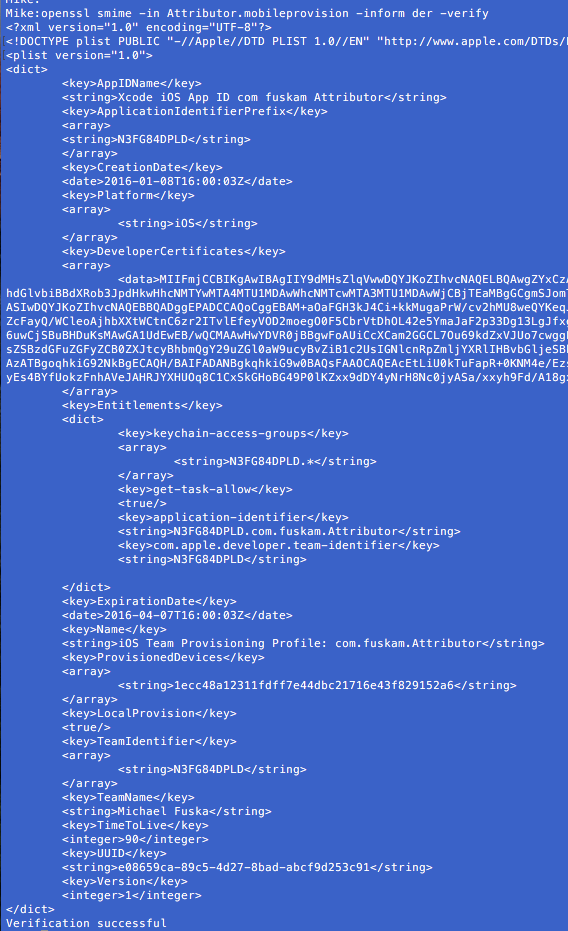
\includegraphics[scale=0.6]{SGML-Format}
        \caption{Provisioning Profile}
        \label{fig:ProvisioningProfile}
\end{figure}

\paragraph{Alle Items eines Provisioning Profile werden nachfolgend aufgelistet}
\begin{enumerate}
% --------APPIDNAME --------------
    \item AppIDName Item

\begin{lstlisting}[captionpos=b, caption={AppIDName Item}]
<key>AppIDName</key>
<string>Xcode iOS appID com fuskam Attributor</string>
\end{lstlisting}
Dieses Item beschreibt den Namen der App inklusive Namespace. (vgl. \cite{iOSSec[5], Hacking[1]})

%-----------------APPLICATIONIDENTIFIERPREFIX ------------------
    \item ApplicationIdentifierPrefix Item
\begin{lstlisting}[captionpos=b, caption={ApplicationIdentifierPrefix Item}]
<key>ApplicationIdentifierPrefix</key>
<array>
    <string>N3FG84DPLD</string>
</array>
\end{lstlisting}
Dieses Item beschreibt den Name der App im Provisioning Portal. Es ist ein zehn Zeichen langer String, welcher im Provisioning Portal generiert worden ist. Der ApplicationIdentifierPrefix wird immer dann erzeugt, wenn eine App ID generiert wird. Dieses Item ermöglicht es Daten zwischen unterschiedlicher Apps zu verteilen. (vgl. \cite{iOSSec[5], Hacking[1]})

%------CREATION DATE --------------
    \item CreationDate Item
\begin{lstlisting}[ captionpos=b, caption={CreationDate Item}]        
<key>CreationDate</key>
<date>2016-01-08T16:00:03Z</date>
\end{lstlisting}
Dieses Item beinhaltet den Zeitstempel der Provisioning Profile Generierung. (vgl. \cite{iOSSec[5], Hacking[1]})

% ----------- PLATFORM --------------------
    \item Platform Item
\begin{lstlisting}[captionpos=b, caption={Platform Item}]        
<key>Platform</key>
<array>
    <string>iOS</string>
</array>
\end{lstlisting}
Dieser Item beinhaltet eine Betriebssystem Liste(Array). Auf diesen Systemen kann die App installiert und ausgeführt werden. (vgl. \cite{iOSSec[5], Hacking[1]})

%------ DEVELOPERCERTIFICATES -----------------------
    \item DeveloperCertificates Item
\begin{lstlisting}[captionpos=b, caption={DeveloperCertificates Item}]        
<key>DeveloperCertificates</key>
<array                
    <data>..... </data>
</array>
\end{lstlisting}
Dieses Item beinhaltet eine Developer Zertifikat Liste(Array). Jedes Zertifikat ist \textit{\glqq base64\grqq{}} codiert. Mit dem \glqq openssl\grqq{} Befehl können alle Attribute des Zertifikats angezeigt werden. (vgl. \cite{iOSSec[5], Hacking[1]}) \newline

\lstset{
    language=bash,
    }
\begin{lstlisting}[captionpos=b, caption={Befehl: openssl -- (Siehe Abbildung: \ref{fig:DeveloperCertificates})}]
openssl x509 -text -in Attributor.pem 
\end{lstlisting}

\begin{figure}[!ht]
        \centering
                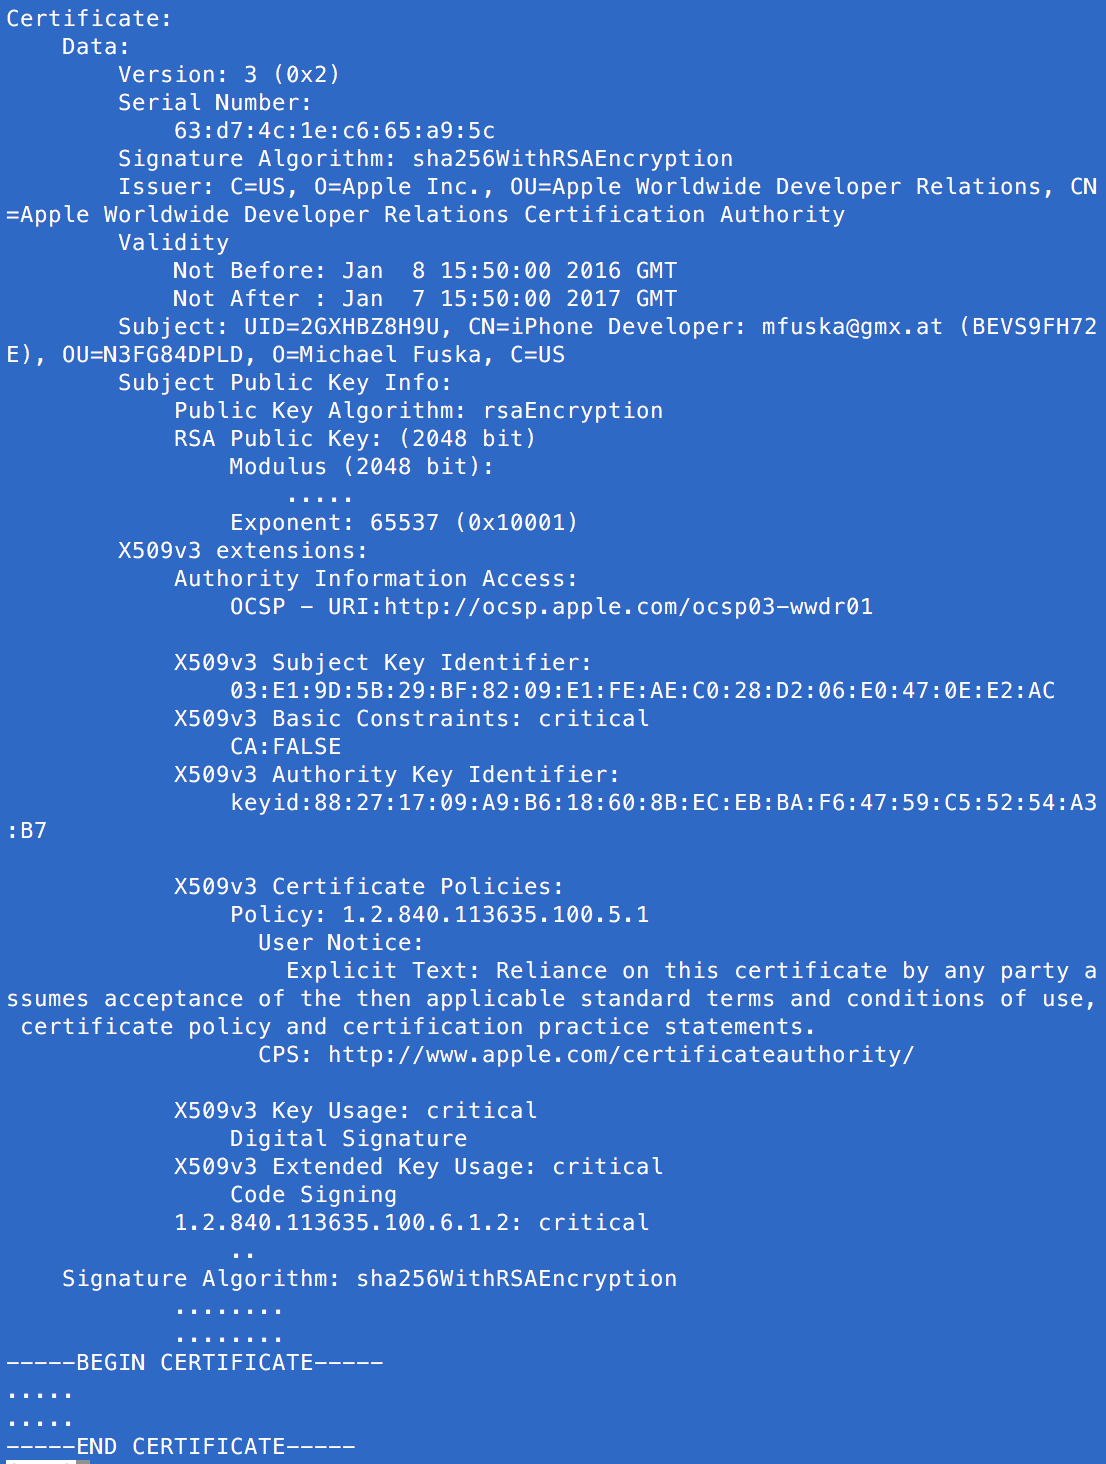
\includegraphics[scale=0.7]{Cert-output}
        \caption{Developer Certificates}
        \label{fig:DeveloperCertificates}
\end{figure}

%-------------ENTITLEMENTS -----------------------
    \item Entitlements Item
\begin{lstlisting}[captionpos=b, caption={Entitlements Item}]
<key>Entitlements</key>
<dict>
    <key>keychain-access-groups</key>
    <array>
        <string>N3FG84DPLD.*</string>           
    </array>
    <key>get-task-allow</key>
    <true/>
    <key>application-identifier</key>
    <string>N3FG84DPLD.com.fuskam.Attributor</string>
    <key>com.apple.developer.team-identifier</key>
    <string>N3FG84DPLD</string>
</dict>
\end{lstlisting}

Nachfolgende werden die möglichen \textit{\glqq Entitlements-Key\grqq{}} beschrieben:

\paragraph{keychain-access-groups:}
Dieses Entitlement verwaltet eine Liste (Array) von ApplicationIdentifierPrefix inklusive Namespace und ist eine Datensicherheit-Mechanismus für Apps. \par 
    \glqq \textit{This entitlement defines an array of strings corresponding to keychains you intend the app to have access to. Each string value in the array are of the format: <prefix>.<bundle\_id>. By default, Xcode creates this entitlement for you a value equal to the application-identifier entitlement. All prefixes in this array of strings must match.}\grqq{} (vgl. \cite{iOSSec[5]} S.8)

\paragraph{get-task-allow:} 
\glqq\textit{This entitlement permits applications signed with the embedded developer certificate to be debugged, indicating that this provisioning profile is intended to permit on-device custom application testing.}\grqq{} (vgl. \cite{iOSSec[5]} S.8) \par 
    \glqq \textit{The boolean value of get-task-allow determines whether Xcode's debugger can attach to the app.}\grqq{} (vgl. \cite{ProvisioningProfile[3]})

\paragraph{application-identifier:} Dieses Entitlement beinhaltet einen eindeutigen Prefix für jede App.\par
    \glqq \textit{The string value of application-identifier is of the format: <prefix>.<bundle\_id> and it corresponds to your app's App ID. Often times the prefix is equal to the Team ID though it isn't always the case. In the provisioning profile, this value includes an asterisk if it is associated to a wildcard App ID. In either case, the application-identifier on an app's signature is always fully qualified to include the app's full bundle ID.} \grqq{} (vgl. \cite{ProvisioningProfile[3]})

\paragraph{task\_for\_pid-allow:} Dieses Entitlement erlaubt es, andere Prozesse zu kontrollieren. 

\paragraph{run-unsigned-code:} Dieses Entitlement erlaubt es, der App nicht signierten Code auszuführen.

%-------- EXPIRATION DATE ----------------------
    \item ExpirationDate Item
\begin{lstlisting}[captionpos=b, caption={ExpirationDate Item}]
<key>ExpirationDate</key>
<date>2016-04-07T16:00:03Z</date>
\end{lstlisting}
Dieses Item legt die Gültigkeit des Provisioning Profile fest. (vgl. \cite{iOSSec[5], Hacking[1]})

% ------- NAME ------------------
    \item Name Item
\begin{lstlisting}[captionpos=b, caption={Name Item}]
<key>Name</key>
<string>iOS Team Provisioning Profile: com.fuskam.Attributor</string>
\end{lstlisting}
Dieses Item definiert den Domain-Namen der App. (vgl. \cite{iOSSec[5], Hacking[1]})

% ----- PROVISIONEDDEVICE ----------------
    \item ProvisionedDevices Item
\begin{lstlisting}[captionpos=b, caption={ProvisionedDevices Item}]
<key>ProvisionedDevices</key>
<array>
    <string>1ecc48a12311fdff7e44dbc21716e43f829152a6</string>
</array>
\end{lstlisting}
Dieses Item beinhaltet eine UDID Liste (Array). Auf den Devices mit diesen UDID kann die App installiert werden. (vgl. \cite{iOSSec[5], Hacking[1]})

%------ LOCALPROVISION -----------
  \item LocalProvision Item
\begin{lstlisting}[captionpos=b, caption={LocalProvision Item}]
<key>LocalProvision</key>
<true/>
\end{lstlisting}

%------ TEAMIDENTIFIER -------------------
    \item TeamIdentifier Item
\begin{lstlisting}[captionpos=b, caption={TeamIdentifier Item}]
<key>TeamIdentifier</key>
<array>
    <string>N3FG84DPLD</string>
</array>
\end{lstlisting}
Dieses Item beinhaltet die Team-ID für welches dieses Provisioning Profile gültig ist.(vgl. \cite{iOSSec[5], Hacking[1]}) \par
\glqq \textit{Your Team ID, which is your team's unique 10-digit alpha/numeric value. This value is often used as the default App ID prefix. Certain features are only allowed across apps whose team-identifier value match, for example, Handoff, keychain and UIPasteboard sharing.}\grqq{} (vgl. \cite{ProvisioningProfile[3]})

%--------- TEAMNAME ------------
    \item TeamName Item
\begin{lstlisting}[captionpos=b, caption={TeamName Item}]
<key>TeamName</key>
<string>Michael Fuska</string>
\end{lstlisting}
 Dieses Item beinhaltet den Teamnamen für welches dieses Provisioning Profile gültig ist. (vgl. \cite{iOSSec[5], Hacking[1]})

%-------------- TIMETOLIVE ----------------------
   \item TimeToLive Item
\begin{lstlisting}[captionpos=b, caption={TimeToLive Item}]
<key>TimeToLive</key>
<integer>90</integer>
\end{lstlisting}
Dieses Item definiert die Gültigkeit des Provisioning Profile in Tagen. Defaultmäßig ist der Wert auf 365 Tage gesetzt. (vgl. \cite{iOSSec[5], Hacking[1]})
 
 %--------- UUID ---------------
    \item UUID Item
\begin{lstlisting}[captionpos=b, caption={UUID Item}]
<key>UUID</key>
<string>e08659ca-89c5-4d27-8bad-abcf9d253c91</string>
\end{lstlisting}
Das Item \textit{\glqq Universally Unique IDentifier\grqq{}} (UUID) identifiziert eine App eindeutig auf einem Device. (vgl. \cite{iOSSec[5], Hacking[1]})

%---------- VERSION -----------------
    \item Version Item
\begin{lstlisting}[captionpos=b, caption={Version Item}]
<key>Version</key>
<integer>1</integer> 
\end{lstlisting}
Dieses Item definiert die Version des Provisioning Profile. Zum heutigen Zeitpunkt ist die Version \textit{\glqq 1\grqq{}} in Verwendung. (vgl. \cite{iOSSec[5], Hacking[1]})
\end{enumerate}

% -------------------------
% -------------------------
\subsection{Signed iOS app}
\label{sec:SignediOSApp}
Mit dem Befehl \glqq codesign\grqq{} (Siehe Listing: \ref{list:codeSignApp}) können die Elemente signierter Apps angezeigt werden, inklusive \textit{\glqq CDHash\grqq{}} und \textit{\glqq CodeDirectory\grqq}.
\newline

\begin{lstlisting}[captionpos=b, caption={Befehl: codesign}, label=list:codeSignApp]
    codesign -dvvv appname
\end{lstlisting}

\begin{description}
    \item[\parbox{\textwidth} {Zwei Werte werden für die Verifikation der Signatur einer App verwendet}]~\par
    \begin{enumerate}
        \item CDHash
        \item CodeDirectory
    \end{enumerate}
\end{description} 

\paragraph{CDHash} ist die Abkürzung für \textit{\glqq Code Directory Hash\grqq{}}. Der CDHash ist ein SHA-1 Hash über die \textit{\glqq Program Code Directory Resource\grqq{}}. Die Code Directory Resource ist das Master Directory des Programm Content. (vgl. \cite{CDHash[1], Debug[1], Debug[2]}) \par

Wie in Kapitel \ref{sec:ProvisioningProfile} beschrieben gibt es drei unterschiedliche Arten wie eine App signiert kann.

Die Abbildung \ref{fig:Developer signed CDHash} zeigt eine App die mit einem Developer Zertifikat signiert wurde. Nur mit dem entsprechenden Provisioning Profile kann die App auf einen iOS Device ausgeführt werden. Das Provisioning Profile muss auf dem iOS Device installiert sein und es muss den \textit{\glqq Public Key des Developer\grqq{}} enthalten.\par 
\begin{figure}[!ht]
        \centering
        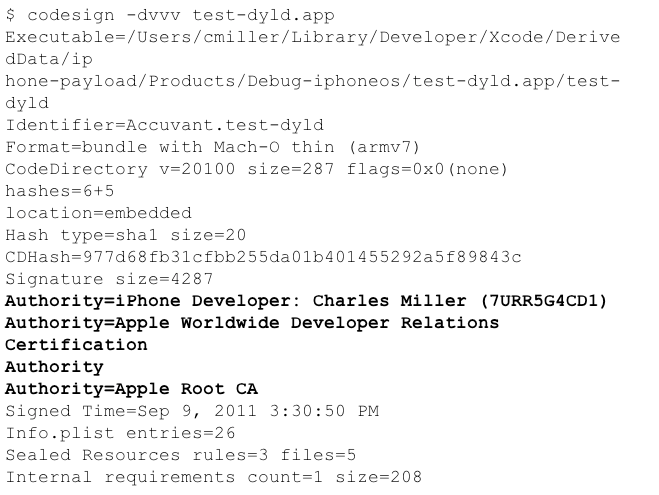
\includegraphics[scale=0.6]{developerZert-codesign-CDHash.png}
        \caption{Developer signed CDHash (vgl. \cite{Hacking[1]})}
        \label{fig:Developer signed CDHash}
\end{figure}

Es besteht immer die Möglichkeit, dass eine App von Apple bzw. einem anderen Entwickler resigniert wird.\cite{Sign[1], Sign[2], Sign[3], Sign[4], Sign[5]}. Die Abbildung \ref{fig:Apple signed CDHash} zeigt eine App die von Apple signiert und via iTunes verteilt wurde.

\begin{figure}[!ht]
        \centering
        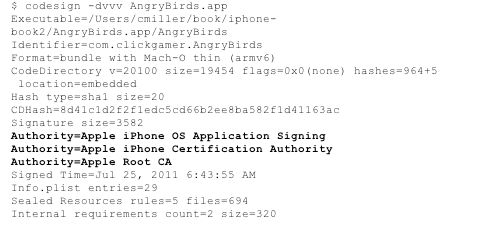
\includegraphics[scale=1.0]{AppleZert_CDHash.png}
        \caption{Apple signed CDHash (vgl. \cite{Hacking[1]})}
        \label{fig:Apple signed CDHash}
\end{figure}

Die Abbildung \ref{fig:Ad-Hoc CDHash} zeigt eine App ohne Informationen betreffend des Zertifikates mit welchen die App signiert wurde. Es ist nur der CDHash verfügbar und das Entitlement adhoc ist gesetzt. Dies bedeutet, dass dieser CDHash im \textit{\glqq static trusted cache\grqq{}} enthalten ist. (vgl. \cite{Sign[1], Sign[2], Sign[3], Sign[4], Sign[5]})

\begin{figure}[!ht]
        \centering
        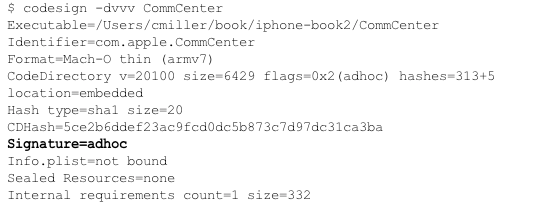
\includegraphics[scale=0.9]{ADhoc_CDHash.png}
        \caption{Ad-Hoc CDHash (vgl. \cite{Hacking[1]})}
        \label{fig:Ad-Hoc CDHash}
\end{figure}

%------------------------------------------------------------------------------
%------------------------------ Encryption and Data Protection
\section{Datenverschlüsselung und -schutz}
\label{sec:EncryptionandDataProtection}

In den Kapiteln zuvor wurden die Sicherheitsmechanismen beschreiben, die sicherstellen, dass nur vertrauenswürdiger Code auf dem Device ausgeführt werden kann. Dieses Kapitel befasst sich mit der Sicherheit von Userdaten auf dem iOS Device. 

Ab der iOS Version 8 wurde die verpflichtende Verschlüsselung von Userdaten eingeführt. Die iOS Produkte verfügen über unterschiedliche Schutzmechanismen, sowohl im Betriebssystem, als auch im iOS Device. Wenn alle anderen Sicherheitsmechanismen umgangen werden, kann trotzdem nicht auf die unverschlüsselten Userdaten zugegriffen werden. Dies ist der Datenverschlüsselung und dem Datenschutz Mechanismus zuzuschreiben.

\subsubsection{Hardware Security Protection}
\label{sec:HardwareSecProtection}

Jedes iOS Device hat eine eigene \textbf{AES 256 Crypto Engine}. Diese Crypto Engine ist Teil der \textit{\glqq Direct Memory Access(DMA) Pathes\grqq{}} und wurde zwischen dem \textit{\glqq Main System Memory\grqq{}} und den \textit{\glqq Flash Memory\grqq{}} eingebaut. Das ermöglicht es, dem iOS Device, die sehr teuren und komplexen kryptographischen Operationen effizient und energiesparend durchzuführen.(vgl. \cite{iOSSec[5], iOSSec[2],iOSSec[1], Apple[4], Apple[5], Apple[6], Apple[3]})

Während der Herstellung des Applikationsprozessors und der Secure Enclave wird die \textit{\glqq Unique device ID\grqq{}} (UID, eindeutige Geräte ID) und die \textit{\glqq device Group ID\grqq{}} (GID, Gerätegruppen ID) in die Hardware gebrannt oder kompiliert.  \par 
Der \textbf{AES 256-Bit Key} besteht aus der UID und der GID. Es ist für keine Software oder Firmware möglich diesen Key direkt auszulesen. Es können nur die Ver- und Entschlüsselung Funktionen verwendet werden, die von der AES Engine zur Verfügung gestellt werden. (vgl. \cite{iOSSec[5], iOSSec[2],iOSSec[1], Apple[4], Apple[5], Apple[6], Apple[3]})

In der \textbf{Secure Enclave} ist ein \textbf{Koprozessor} des \textit{\glqq Apple A7 Prozessors\grqq{}} und des späteren \textit{\glqq A-Serie Prozessors\grqq}. Jede Secure Enclave hat ihre eigene UID, die bei der Herstellung des Koprozessors in diesen gebrannt wird. Es werden in der Secure Enclace die verschlüsselten biometrischen Daten (Fingerprint) des User gespeichert. Unter anderen findet auch die Verifikation des AES 256 verschlüsselten User Passcodes in der Secure Enclave statt. Alle anderen kryptographischen Keys werden vom  \textit{\glqq Random Number Generator(RNG)\grqq{}} erzeugt. Der RNG basiert auf dem \textit{\glqq AES 256 CTR\_DRBG Algorithmus\grqq{}}.(vgl. \cite{iOSSec[5], iOSSec[2],iOSSec[1], Apple[4], Apple[5], Apple[6], Apple[3]})

Durch die Verschachtelung der UID mit dem AES 256-Bit Key, ist es nicht möglich, den Flash Memory in ein anderes iOS Device einzubauen und dann die Userdaten zu dekodieren. Somit können die Userdaten nur auf dem Device mit dem Koprozessor mit der entsprechenden UID entschlüsselt werden. (vgl. \cite{iOSSec[5], iOSSec[2],iOSSec[1], Apple[4], Apple[5], Apple[6], Apple[3]})

\subsubsection{Datenschutz}
\label{sec:DataProtection}

Zusätzlich zur Hardware Protection stellt Apple eine weiter Sicherheitstechnologie für iOS Geräte zur Verfügung, dies wird \textbf{Data Protection}(Datenschutz) genannt. Ab der iOS Version 7.0 wird Data Protection für alle Third-Party Apps defaultmäßig aktiviert.(vgl. \cite{iOSSec[5], iOSSec[2],iOSSec[1], Apple[4], Apple[5], Apple[6], Apple[3]})

\paragraph{Datenschutz} wurde spezielle für mobile Geräte entwickelt. iOS entschlüsselt immer nur die Daten die gerade von Apps/Prozessen verwendet/benötigt werden. Dies hat den Vorteil, dass bei einem Event (zB. eingehender Anruf) nicht, die gesamte Daten entschlüsselt werden müssen, um diesen Event behandeln zu können. (vgl. \cite{Apple[4]})

\paragraph{File Datenschutz} basiert auf dem Datenschutz-Mechanismus, dieses wiederum beruht auf einer hierarchischen Schlüsselverteilung. Mit dem Erstellen eines neuen Files auf der Datenpartition, wird auch ein neuer \textit{\glqq File Key 256-Bit\grqq{}} (\glqq Per-File Key\grqq) erzeugt. Dieser wird der Hardware AES Engine übergeben und dieser wird dann zur Verschlüsselung des Files verwendet.  Der \textit{\glqq AES-CBC Mode\grqq{}} wird verwendet um das File auf den Flash Memory zu schreiben. Der A8 Prozessor verwenden hierfür den \textit{\glqq AES-XTS Mode\grqq{}}.  \par
Der \textbf{Initialisierungsvektor(IV)} wird mit Hilfe des Block Offset der Datei berechnet und zur Verschlüsselung wird der SHA-1 des \textit{\glqq File Keys\grqq{}} verwendet. (vgl. \cite{iOSSec[5], iOSSec[2],iOSSec[1], Apple[4], Apple[5], Apple[6], Apple[3]})

Der Content des Files wird mit dem \textbf{File Key} verschlüsselt. Dieser wird mit einem \textbf{Class Key} verpackt (wrapped) und in den Metadaten des Files gespeichert. Die Metadaten werden mit dem \textbf{File System Key} verschlüsselt. Der Class Key ist mit dem \textbf{Hardware Key} geschützt und für mache Klassen zusätzlich noch mit \textbf{Passcode Key}.(vgl. \cite{iOSSec[5], iOSSec[2],iOSSec[1], Apple[4], Apple[5], Apple[6], Apple[3]})
\begin{figure}[!ht]
        \centering
        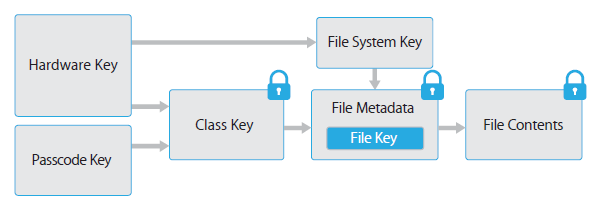
\includegraphics[scale=0.9]{fileDataProtection.PNG}
        \caption{File Data Protection (\cite{Apple[4]} S.11)}
        \label{fig:FileDataProtection}
\end{figure}

\subsubsection{Passcode}
\label{sec:Passcode}

Mit dem aktiveren das Passcodes wird der Datenschutz des iOS Devices aktiviert. 
\begin{description}
    \item[\parbox{\textwidth} {Der User hat die Möglichkeit zwischen drei Einstellungsvarianten des Passcodes zu variieren}]~\par
   \begin{enumerate}
        \item eine vierstellige Zahl,
        \item eine sechsstellige Zahl und
        \item eine beliebige Anzahl alphanumerischer Zeichen.
    \end{enumerate}
\end{description} 

Die Sicherheit des iOS Devices hängt mit der Sicherheit des Passcodes zusammen. Je stärker der Passcode ist umso stärker ist auch der Verschlüsselungskey. 

\subsection{Sandbox}
\label{sec:Sandbox}

\textbf{Die Sandbox} ist ein weiterer Zugriffkontrollmechanismus um Userdaten zu schützen. Die Sandbox wird auch als \textbf{Last Line of Defense} bezeichnet. Wenn alle anderen Sicherheitsmechanismen schon versagt haben, verhindert die Sandbox ein übergreifen der Schadsoftware auf das gesamte Device. Die Schadsoftware kann sich nur in den Verzeichnissen der App ausbreiten. Die Malware kann nur auf die Daten in diesem Verzeichnisbaum zugreifen und es stehen auch nur die Systemressourcen zur Verfügung, die für diese App vom Entwickler festgelegt wurden. \par
Würde eine Schadsoftware Zugriff auf eine App erhalten die in keiner Sandbox läuft, so hätte die Malware Zugriff auf alle Daten des Devices und könnte alle Systemressourcen uneingeschränkt verwenden.

\begin{description}
    \item[\parbox{\textwidth} {Unteranderem könnte die Malware folgende Systemressourcen unbemerkt vom User verwenden}]~\par
    \begin{itemize}
        \item die eingebaute Kamera
        \item das eingebaute Mikrophon
        \item die Network Sockets
        \item und auf die meisten Bereiche des File Systems.
    \end{itemize}
\end{description} 
(vgl. \cite{Apple[6], Sandbox[1], Sandbox[2],Sandbox[3], Sandbox[4], Sandbox[5]})

\begin{figure}[!ht]
        \centering
                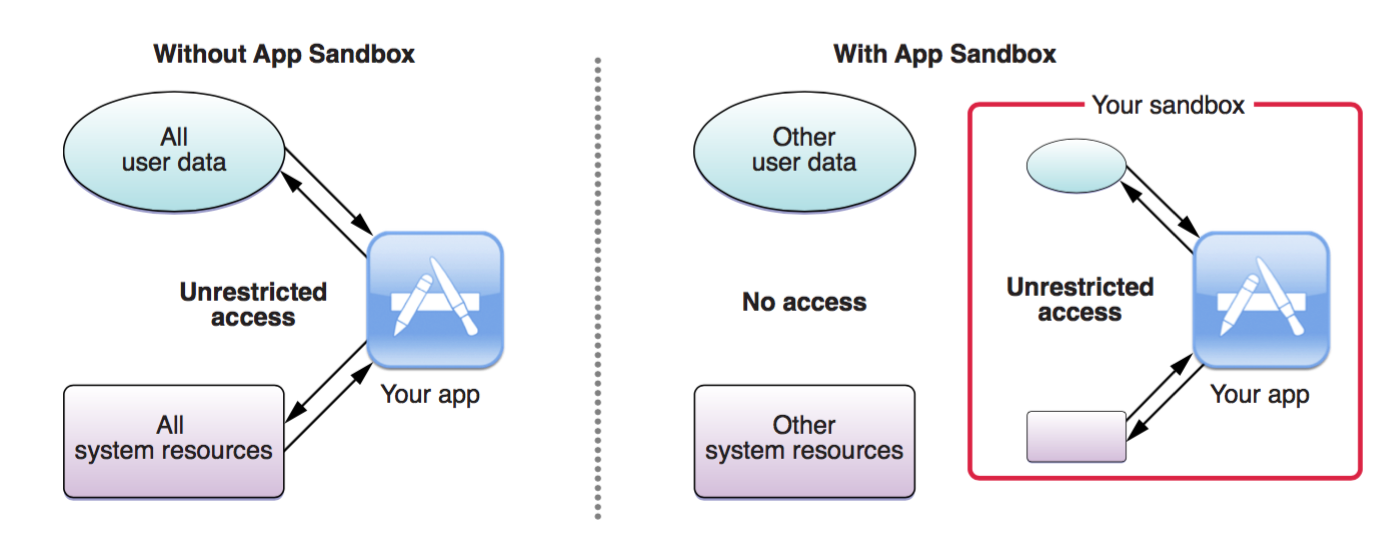
\includegraphics[scale=0.6]{iOSsandbox}
        \caption{iOS Sandbox (vgl. \cite{Sandbox[3]}, S.6)}
        \label{fig:iOSsandbox}
\end{figure}

\begin{description}
    \item[\parbox{\textwidth} {Wenn eine Sandbox für eine App vom iOS angelegt wird, stehen der App folgende Container Verzeichnisse zur Verfügung}]~\par
    \begin{enumerate}
        \item \textbf{ App Container Directory:} \\
        Beim ersten Starten der App wird vom Betriebssystem ein Verzeichnis erstellt, dieses kann nur von dieser App verwendet werden. Dies wird als Container bezeichnet. Jeder User des Systems erhält seinen eigenen Container für diese App.
        \item \textbf{ App Group Container Directory:} \\
        Mit Hilfe von Entitlements kann konfiguriert werden, welches Apps Zugriff auf den Group Container haben. Dieser Container dient zum Datenaustausch zwischen unterschiedlichen Apps.
        \item \textbf{Diverse System Verzeichnisse}
    \end{enumerate}
\end{description} 


%\subsection{Schutzklassen}
%\label{sec:Schutzklassen}

%\subsection{Remote Wipe}
%\label{sec:RemoteWipe}

%\subsection{Collecting Signing}
%\label{sec:CollectingSigning}

%\subsection{Verifying Signing}
%\label{sec:VerifyingSigning}

%\subsection{Dynamic Code Signing}
%\label{sec:DynamicCodeSigning}

%\subsection{Runtime Process Security}
%\label{sec:RuntimeProcessSecurity}



%------------------------------------------------------------------------------
%------------------------------  Stack Guard ----------------------------------
%\section{Stack Guard}
%\label{sec:StackGuard}
%\subsection{Stack}
%\label{sec:Stack}
%\subsection{Heap}
%\label{sec:Heap}
%
%------------------------------------------------------------------------------
%------------------------------  NetworkSecurity
%\section{Network Security}
%\label{sec:NetworkSecurity}
%
%\subsection{Secure Socket Layer}
%\label{sec:SSL}
%
%\subsection{Transport Layer Security}
%\label{sec:TLS}
